\documentclass[%
%draft,
%submission,
%compressed,
final,
%
%technote,
%internal,
%submitted,
%inpress,
reprint,
%
%titlepage,
notitlepage,
%anonymous,
narroweqnarray,
inline,
twoside,
invited
]{ieee}
\usepackage[utf8]{inputenc}
\usepackage[spanish]{babel}
\usepackage{graphicx}
\usepackage{verbatim}
\usepackage{moreverb}
\usepackage{amsmath}
\usepackage{amsfonts}
\usepackage{amssymb}
\usepackage{fancybox}
\usepackage{float}
\usepackage{fancyvrb}
\usepackage{subfigure}
\newcommand{\latexiie}{\LaTeX2{\Large$_\varepsilon$}}
%\usepackage{ieeetsp} % if you want the "trans. sig. pro." style
%\usepackage{ieeetc} % if you want the "trans. comp." style
%\usepackage{ieeeimtc} % if you want the IMTC conference style
% Use the `endfloat' package to move figures and tables to the end
% of the paper. Useful for `submission' mode.
%\usepackage {endfloat}
% Use the `times' package to use Helvetica and Times-Roman fonts
% instead of the standard Computer Modern fonts. Useful for the
% IEEE Computer Society transactions.
%\usepackage{times}
% (Note: If you have the commercial package `mathtime,' (from
% y&y (http://www.yandy.com), it is much better, but the `times'
% package works too). So, if you have it...
%\usepackage {mathtime}
% for any plug-in code... insert it here. For example, the CDC style...
%\usepackage{ieeecdc}

\begin{document}

%----------------------------------------------------------------------
% Title Information, Abstract and Keywords
%----------------------------------------------------------------------
\title[JPEG: Compresión de Imágenes]{%
JPEG y la compresión de imágenes\\ mediante DCT Quantization}

% format author this way for journal articles.
% MAKE SURE THERE ARE NO SPACES BEFORE A \member OR \authorinfo
% COMMAND (this also means `don't break the line before these
% commands).
\author[Sturla, Sneidermanis]{Martín Sturla, Darío Sneidermanis\\\textit{Estudiantes 
       Instituto Tecnológico de Buenos Aires (ITBA)}\\
\\\textbf{31 de Mayo de 2012}
}



\journal{Cátedra\ de\ Met.\ Num.\ Avanzados,\ ITBA\ }
\titletext{- 31, MAYO\ 2012}
\ieeecopyright{\copyright\ 2011 ITBA}
\lognumber{}
\pubitemident{}
\loginfo{31 de Mayo, 2012.}
\firstpage{1}

\confplacedate{Buenos Aires, Argentina, 31 de Mayo, 2012}

\maketitle               

\begin{abstract} 
El siguiente paper busca analizar la compresión de imágenes utilizando \textit{DCT Quantization} según 
la especificación JPEG original, comparando el nivel de compresión alcanzado y calidad perdida 
utilizando distintos niveles de cuantización.
\end{abstract}

\begin{keywords}
JPEG, compresión de imágenes, transformada discreta coseno, cuantización.
\end{keywords}

%----------------------------------------------------------------------
% SECTION I: Introduccion%----------------------------------------------------------------------
\section{Introducción}

\par Históricamente la compresión de datos siempre ha sido de notable interés para la informática,  
ya sea para guardar un archivo en algún dispositivo de capacidad limitada o para enviar un 
archivo por algún enlace utilizando la menor cantidad de banda ancha posible.
 Debido a estos requerimientos, surgen los primeros programas que haciendo uso de técnicas de compresión de datos, 
 por ejemplo \textit{Run Length Encoding} o 
codificación de \textit{Huffman}, comprimen y descomprimen archivos. Algunos ejemplos incluyen 
\textit{Winzip}, lanzado en 1991, o \textit{Winrar}, lanzado en 1993. Sin embargo en el caso de las imágenes, 
debido a la naturaleza de sus datos, existen mejores alternativas para comprimirlas. Ya en el año 1992, 
un comité conocido como \textit{Join Photographic Experts Group} comienza a publicar pautas 
para la compresión de imágenes, conocidas como la especificación \textit{JPEG}. 
\par La especificación original de JPEG, en la cual se centra este trabajo, indica que la compresión de las 
imágenes consiste en dos etapas fundamentales: una codificación con pérdida de información,  
seguida de una compresión sin pérdida, como por ejemplo las dos ya mencionadas. En esta primer etapa 
existen dos maneras de reducir la información: \textit{chroma subsampling} y \textit{DCT Quantization}. La primera, 
la cual no es analizada en este trabajo, consiste en aprovechar que el ojo humano tiene una menor agudeza 
para diferenciar colores que brillantez o \textit{luma}, por lo cual se reduce la resolución de la croma. La segunda 
consiste en hacer uso de que el ojo humano es capaz de diferenciar cambios de 
luma en zonas grandes, pero no tan tenazmente en zonas pequeñas. Debido a esto, se eliminan estas componentes 
de frecuencia espaciales altas en zonas pequeñas (casi imperceptibles para el ojo) y se suavizan los 
cambios de luma (también se efectúa un proceso similar con la croma). Debido a esta eliminación de información, 
existe mayor redundancia de los datos, por lo que un llamado posterior a un algoritmo de compresión será más 
efectivo.
\par El objetivo primordial del trabajo es analizar la técnica de \textit{DCT Quantization} para distintas 
imágenes y matrices de cuantización, analizando en cada caso la tasa de compresión, el error introducido a la 
imagen recuperada y su distorsión gráfica. La sección 2 explica en profundidad la primer etapa de la compresión. 
La sección 3 trata sobre la segunda etapa de compresión. La sección 4 explica brevemente cómo recuperar 
la imagen. La sección 5 contiene los resultados.

%----------------------------------------------------------------------
% SECTION II: Marco Teórico
%----------------------------------------------------------------------

\section{Etapa de compresión con pérdida de información}

\subsection{Transformación del espacio de colores}

\par La primer etapa de compresión se centra en el manejo de luma y croma, por lo cual es necesario transformar 
los datos de las imágenes, que normalmente contienen la cantidad de rojo, verde y azul en cada pixel (\textit{RGB}). 
Estos datos son transformados a luma en un canal, $Y^{'}$, y crominancia en dos: $C_B$ y $C_R$. Estos últimos 
 representan la proporción de verde con respecto al azul y rojo, respectivamente. 
 Este cambio es también útil dado que la luma se concentra 
en sólo un canal (en \textit{RGB} está disperso entre los tres). Dado que la luma es el componente más 
importante para el ojo humano, se puede hacer una mayor compresión de datos.

\par Las componentes $Y^{'}C_BC_R$ son una combinación lineal de las componentes $RGB$. Las siguientes ecuaciones 
 muestran más en profundidad la naturaleza de la conversión.

\[
 \begin{pmatrix} Y^{'} \\ C_B \\ C_R \end{pmatrix} = \begin{pmatrix} +0.2990 & +0.5870 & +0.1140 \\
-0.1687 & -0.3313 & +0.5000 \\
+0.5000 & -0.4187 & -0.0813  \end{pmatrix} \begin{pmatrix}R \\ G \\ B\end{pmatrix} + \begin{pmatrix}0 \\ 128 \\ 128\end{pmatrix}
\]

\[
 \begin{pmatrix} R \\ G \\ B \end{pmatrix} = \begin{pmatrix} +1.00000 & +0.00000 & +1.40200 \\
+1.00000 & -0.34414 & -0.71414 \\
+1.00000& +1.77200 & +0.00000  \end{pmatrix}  \begin{pmatrix}Y^{'} \\ C_B - 128\\ C_R - 128\end{pmatrix}
\]


\subsection{Separación en bloques}

\par Luego de la transformación a los canales $Y^{'}C_BC_R$, la imágen se debe separar en bloques, que representan 
las pequeñas zonas en las cuales se desea eliminar las frecuencias altas de luma y croma. El tamaño de los bloques 
depende de la tasa de submuestreo de croma usada, y varía entre cuadrados de 8 pixeles y 16 pixeles. Dado que 
no se utilizó submuestreo, se utilizaron bloques de 8.
\par En el caso de que las dimensiones de la imágen no sean múltiplos del tamaño del bloque, se procede a extenderla 
hasta que los bloques quepan perfectamente. Los nuevos pixeles son llenados utilizando información de sus vecinos más 
inmediatos. Otras alternativas analizadas incluyen llenar los canales de los nuevos pixeles con 0.

\subsection{Transformación del Coseno Discreta}

El siguiente paso consiste en transformar los valores de los canales en cada bloque a sus 
frecuencias espaciales en dos dimensiones, 
utilizando la transformación del coseno discreta de tipo II. Esta última consiste en una transformada 
de Fourier discreta utilizando únicamente cosenos. Para una cierta matriz cuadrada, la transformada está 
dada por la ecuación:

\begin{equation}
	G_{u, v} = \sum^{N-1}_{x=0}\sum^{N-1}_{y=0}\frac{\alpha(u)\alpha(v)}{N}g_{x, y}\cos(\frac{\pi}{8}(x+\frac{1}{2})u)cos(\frac{\pi}{8}(y+\frac{1}{2})v)
\end{equation}

Donde $g_{x, y}$ representa el elemento de la fila $x$ y la columna $y$ del bloque de entrada, y $G_{u, v}$ 
el elemento de la fila $u$ y columna $v$ de la matriz de frecuencias de salida.

Análogamente la antitransformada está dada por:

\begin{equation}
	g_{x, y} = \sum^{N-1}_{u=0}\sum^{N-1}_{v=0}\frac{\alpha(u)\alpha(v)}{N}G_{u, v}\cos(\frac{\pi}{8}(x+\frac{1}{2})u)cos(\frac{\pi}{8}(y+\frac{1}{2})v)
\end{equation}

En ambas ecuaciones:

\begin{equation}
	\alpha(k) = \left \{
		\begin{array}{rl}
			1 & \mbox{si } k = 0 \\ 
			\sqrt{2} & \mbox{en otro caso} \\
		\end{array}
		\right.
\end{equation}

\par Nótese que los coeficientes de las frecuencias más bajas se encuentran en los valores bajos de $x$ e $y$, 
es decir en la zona superior 
izquierda de la matriz de frecuencias. Similarmente los coeficientes de las frecuencias más altas se encuentran 
en la zona inferior derecha. Esta transformación concentra la señal de entrada en las frecuencias espaciales más bajas, 
es decir en la zona superior izquierda. En particular, comúnmente el mayor valor en módulo es $G_{0,0}$. 
Este valor representa la frecuencia con valor 0, y por lo tanto es en esencia un promedio de los 64 valores de entrada
 (con ciertas modificaciones, dado que se divide por $N$ y no por $N^{2}$, y hay valores con mayor peso). A este 
valor se lo llama $DC coefficient$ dado que en circuitos el promedio de una señal ( es decir el valor asociado 
a la frecuencia cero) es la corriente efectiva directa ($DC$). Al resto de los valores se los llama $AC$ debido 
a que representan la componente alterna de la corriente. La transformada discreta del coseno tiende a 
concentrar la señal en las frecuencias espaciales más bajas (ver anexo D).


\par También es importante destacar que los valores de los canales son llevados a un rango 
alrededor del $0$ antes de ser transformados, en el intervalo $[-127,128]$. Esto se logra fácilmente restando 
$127$ a todos los valores de entrada.

\subsection{Cuantización}

\par El paso final de la primer etapa de compresión, y el mayor responsable de la pérdida de información, es la cuantización 
de la matriz de coeficientes de frecuencias. Este paso consiste en dividir cada elemento de dicha matriz por un elemento de una  
matriz de cuantización, y redondear el valor obtenido. 
Las matrices de cuantización sugeridas por la especificación JPEG son las siguientes:

\( Qy = 
\begin{pmatrix}
16 & 11 & 10 & 16 & 24 & 40 & 51 & 61 \\
12 & 12 & 14 & 19 & 26 & 58 & 60 & 55 \\
14 & 13 & 16 & 24 & 40 & 57 & 69 & 56 \\ 
14 & 17 & 22 & 29 & 51 & 87 & 80 & 62 \\ 
18 & 22 & 37 & 56 & 68 & 109 & 103 & 77 \\
24 & 35 & 55 & 64 & 81 & 104 & 113 & 92  \\ 
49 & 64 & 78 & 87 & 103 & 121 & 120 & 101 \\
72 & 92 & 95 & 98 & 112 & 100 & 103 & 99 \\ 
\end{pmatrix}\)
\par
\( Qc = 
\begin{pmatrix}

17 & 18 & 24 & 47 & 47 & 99 & 99 & 99 \\
18 & 21 & 26 & 26 & 66 & 99 & 99 & 99 \\
24 & 26 & 56 & 99 & 99 & 99 & 99 & 99 \\ 
47 & 66 & 99 & 99 & 99 & 99 & 99 & 99 \\ 
99 & 99 & 99 & 99 & 99 & 99 & 99 & 99 \\
99 & 99 & 99 & 99 & 99 & 99 & 99 & 99 \\
99 & 99 & 99 & 99 & 99 & 99 & 99 & 99 \\
99 & 99 & 99 & 99 & 99 & 99 & 99 & 99 \\
\end{pmatrix}\)

La fórmula para obtener los valores es la siguiente:

\begin{equation}
\label{eqCuantizacion}
\mathbf{B}(k,l)=round\left(\frac{\mathbf{A}(k,l)}{\mathbf{Q}_Y(k,l)}\right)
\end{equation}

\par En otras palabras, se divide cada elemento de la matriz de coeficientes de frecuencas por su elemento 
correspondiente de la matriz de cuantización y se redondea. Para la luma se utiliza $\mathbf{Q}_Y(k,l)$ y para 
croma $\mathbf{Q}_c(k,l)$.
\par Nótese que existen varios valores de entrada que son transformados a la misma salida, es decir la relación 
no es inyectiva. Debido a esto, se pierde información. En particular, dado un coeficiente $k$ de la matriz 
de cuantización, existe un intervalo de longitud $k$ que producirá la misma salida. Ergo, 
valores más grandes de la matriz de cuantización implican una mayor pérdida de información. Si se observan ambas 
matrices con detenimiento, se puede apreciar que los valores son mayores en la zona inferior derecha. Esto 
implica que la mayor pérdida de información ocurre en las frecuencias altas de los canales, que es lo que se 
buscaba en un principio.  Asimismo, debido a que la transformada coseno discerta concentra la señal en la zona 
superior izquierda, y los coeficientes de cuantización son mayores en la zona inferior derecha, el resultado de la 
cuantización tendrá una densidad de ceros considerable en esta última zona (referirse al anexo D para ver ejemplos).



\par Se decidió además experimentar con distintas matrices de cuantificación. Para ello se multiplicó a las 
matrices estándares de cuantización por un cierto valor $\alpha$.

\section{Codificación entrópica}

\subsection{Reordenamiento y codificación}

\par La segunda etapa de la compresión consiste en aplicar una codificación entrópica a los datos cuantizados. Debido 
a la gran densidad de ceros producida por la transformación y cuantización, este tipo de algoritmos logra 
una compresión más efectiva. La especificación JPEG admite dos algoritmos: la codificación de \textit{Huffman} y 
codificación aritmética. Ambos consisten en sustituir instancias de patrones frecuentes por cadenas de bits 
más cortas, con la diferencia que \textit{Huffman} reemplaza cada patrón de entrada por su código respectivo, 
mientras que la aritmética lo transforma en un numero real. La codificación aritmética por lo general obtiene 
resultados entre 5 y 7\% más compactos, pero por lo general se utiliza \textit{Huffman} debido a problema de patentes 
y su mayor velocidad.
\par Sin importar qué algoritmo se utilice, la gran densidad de ceros se traduce a que existe un patrón extremadamente 
frecuente, el cual puede ser reemplazado por una cadena de bits particularmente corta para reducir el tamaño del 
archivo. Sin embargo, se pueden modificar algunos datos para reducir aún más la tasa de compresión.
\subsubsection{Reordenamiento}

\par Antes de ejecutar el algoritmo de codificación, se pueden reordenar los valores de la matriz cuantificada, 
ordenando los valores según qué frecuencia representan. 

\begin{figure}[H]
	\begin{center}
	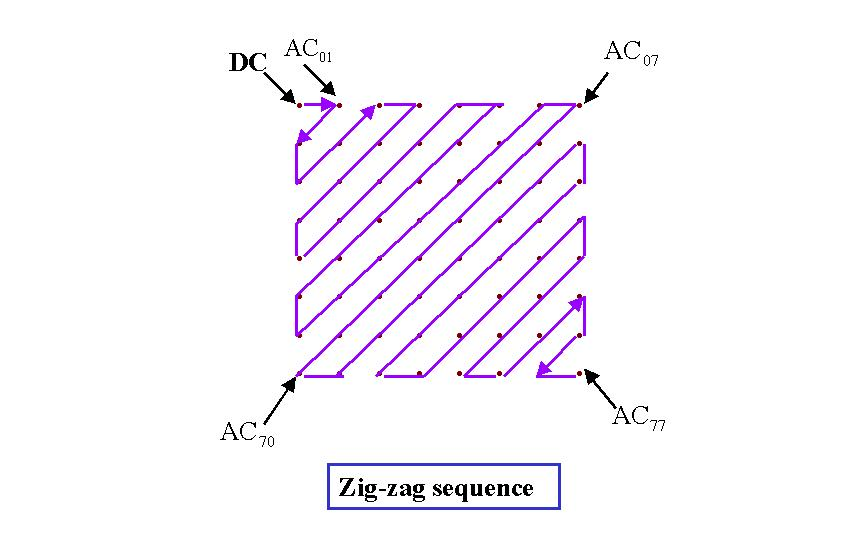
\includegraphics[scale=0.5]{./img/zig-zag.jpg}
	\end{center}
\end{figure}
\begin{center}
\par Figura 1: Reordenamiento de los valores según su frecuencia
\end{center}

\par Debido a que los valores asociados a mayores frecuencias son mayormente cero, este reordenamiento casuará 
cadenas largas de ceros en los datos antes de codificar. Esto resulta en una codificación más compacta. Además, 
por lo general se codifica un símbolo especial indicando que el resto del bloque está únicamente conformado 
por ceros.

\subsubsection{Resta del coeficiente DC}

El valor $DC$ suele ser el mayor valor de cada bloque. Si se pueden acotar los valores de los bloques a un intervalo 
pequeño en un entorno del 0, la codificación sería más eficaz. Para eliminar los valores altos de $DC$, se puede hacer 
uso de que el $DC$ representa el promedio de los canales de un bloque. Asumiendo una imagen normal, es muy posible 
que el promedio de los canales en pixeles adyacentes sea similar. Debido a esto, en vez de guardar el $DC$ se puede 
guardar la diferencia entre el $DC$ actual y el del pixel anterior. Esto reduciría la cantidad de valores 
posibles (pudiendo incrementar incluso la frecuencia de ceros marginalmente).

\subsection{Cálculo de cota superior razonable}

\par Para hallar una cota superior razonable y simple al tamaño del archivo resultante luego de la compresión,
 se puede 
utilizar la frecuencia relativa de valores de canales de pixeles con valor en 0. 
Utilizando una codificación de \textit{Huffman}, 
se le podría asignar a estos pixeles un único bit, en 0. En el peor de los casos, el resto de los valores 
varía uniformemente entre $-127$ y $128$ (es muy difícil que los valores superen estas magnitudes tras 
la cuantificación), por lo cual se necesitan 9 bits para almacenarlos (un 1 seguido 
de la representación binaria del número).
\par En la imagen original, se utilizan $24$ bits por pixel, $8$ por cada canal. Asumiendo que $p$ es la frecuencia 
de valores de canales en 0, es fácil verificar que en promedio pixel necesitará:

\begin{equation}
b_{pixel}=3(p+9(1-p))
\end{equation}

\par Es fácil ver también que para valores de $p$ mayores a $\frac{1}{8}$ ya se usan menos de $24$ bits (nótese sin 
embargo que para valores tan bajos de $p$ seguramente haya una mejor codificación que la asumida; esta última asume 
valores más cercanos a $1$ de $p$, como se observa en la práctica). Con un valor de $0.9$, por ejemplo, esta cantidad 
se reduce a $5.4$ bits.
\par Nótese que esta es simplemente una cota superior razonable. Utilizando restas de coeficientes $DC$ y reordenamientos 
la cantidad de bits seguramente será menor. La estimación no contempla el espacio requerido por la tabla de codificaciones 
que se guarda en el encabezado del archivo. Este se puede despreciar asumiendo que la imagen posee dimensiones considerables.



\section{Procedimiento de recuperación}

En esencia el procedimiento de recuperación consiste en los mismos pasos ya nombrados pero aplicados 
en orden inverso. Primero se descomprime utilizando la descodificación entrópica. Se multiplican 
los valores de cada bloque por su valor correspondiente en la matriz de cuantificación. Se aplica la 
antitransformada discreta del coseno a cada bloque, y luego se recupera la imagen en los canales luma y croma 
con los bloques. Finalmente se transforman dichos canales a los canales $RGB$.

\section{Resultados y conclusiones}

\subsection{Tipos de imágenes}

\par Como se puede observar en la Tabla 1 en el anexo C, la codificación alcanza valores cercanos o superiores al $90\%$ de 
ceros en la imagen. Según la estimación planteada, esto reduce la cantidad de bits por pixel 
 a valores entre $4$ y $6$. Asimismo, se puede observar que el error es más de tres veces mayor en las imágenes de tipo 
íconos, es decir alguna forma o figura sobre un fondo blanco, como el logo de \textit{Facebook} o \textit{Chrome}.
 Esto se debe a que en la frontera entre dicha figura y el fondo existen cambios bruscos de luminosidad, 
 que serán suavizados en la codificación. Esto incrementa el error cuadrático medio y hace que 
 el contorno de la figura se distorsione. El error en el logo de \textit{Chrome} es aún mayor, debido a ser  
 circular. Dado que el algoritmo codifica en ventanas cuadradas, se puede esperar aún más distorsiones 
 en el límite de la figura. En imágenes que representan fotografías de paisajes estos fenómenos no se 
 encuentran habitualmente, por lo que se puede verificar que el error cuadrático medio es menor.



\subsection{Variaciones en la cuantización}

\par En la tabla 2 en el anexo C se puede verificar que si se utilizan matrices de cuantificación con valores mayores 
( es decir mayor $\alpha$) el error sube, pero la densidad de ceros lo hace también. Por otro lado para 
valores menores de $\alpha$, tanto el error como la densidad de ceros disminuye.




\subsection{Dimensiones indivisibles por 8}

Para llevar una imagen a bloques cuyas dimensiones no son múltiplos de 8, se deben agregar pixeles. La 
tabla 3 en el anexo C muestra la diferencia entre el rellenado de dichos pixeles con ceros y el rellenado usando 
el pixel del borde más cercano.


\par Se puede verificar que si se rellena con ceros, el borde de la imagen presenta distorsiones de los 
colores verdes y magenta (ver figuras 2 y 3).

\begin{figure}[H]
	\begin{center}
	
\includegraphics[scale=3]{./img/facebookout.png}
	\end{center}
\end{figure}
\begin{center}
\par Figura 2: Rellenado usando pixel del borde. Imagen ampliada, factor 3. Factor $\alpha=1$.
\end{center}

\begin{figure}[H]
	\begin{center}
	
\includegraphics[scale=3]{./img/facebookout0.png}
	\end{center}
\end{figure}
\begin{center}
\par Figura 3: Rellenado usando ceros. Imagen ampliada, factor 3. Factor $\alpha=1$.
\end{center}

\subsection{Bloques en ampliaciones de imagenes}

Si se amplía la imagen lo suficiente, se puede ver la división de bloques ocurrida (ver figura 4 o Anexo A).

\begin{figure}[H]
	\begin{center}
	
\includegraphics[scale=3]{./img/chrome3out.png}
	\end{center}
\end{figure}
\begin{center}
\par Figura 4: Logo de \textit{chrome} ampliado con un factor de 3. Factor $\alpha=3$ para hacer más vistosos los bloques.
\end{center}


\vspace{0.4cm}


\begin{thebibliography}{1}


\bibitem{lamport1}
\newblock {\em{  JPEG - http://en.wikipedia.org/wiki/Jpg}}
\bibitem{lamport1}
\newblock {\em{ Codificación Huffman - http://en.wikipedia.org/wiki/Huffman\_coding}}
\bibitem{lamport1}
\newblock {\em{ Coeficiente DC - http://en.wikipedia.org/wiki/DC\_Bias}}
\bibitem{lamport1}
\newblock {\em{http://www.cmlab.csie.ntu.edu.tw/cml/dsp/training/coding/jpeg/jpeg/encoder.htm}}

\end{thebibliography}




\clearpage

\onecolumn

\section*{Anexo A: Imagenes y sus codificaciones. Factor $\alpha = 1$ en todos los casos.}

\begin{figure}[H]
	\begin{center}
	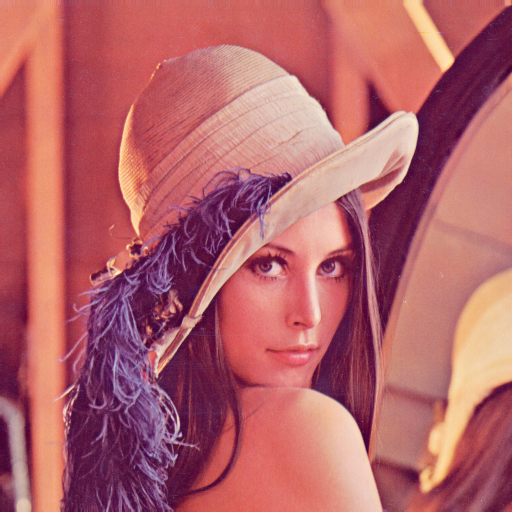
\includegraphics[scale=0.7]{./img/lenacolor.png}
	\end{center}
\end{figure}
\begin{center}
\par Figura 5: Imagen de Lenna de 512x512 pixeles.
\end{center}

\begin{figure}[H]
	\begin{center}
	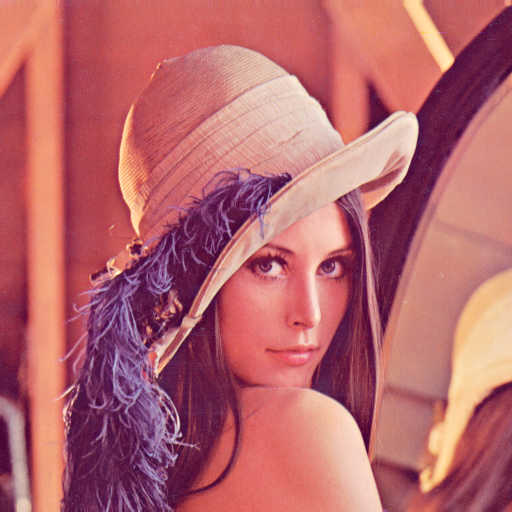
\includegraphics[scale=0.7]{./img/lenaout.png}
	\end{center}
\end{figure}
\begin{center}
\par Figura 6: Imagen de Lenna de 512x512 pixeles tras codificar.
\end{center}

\begin{figure}[H]
	\begin{center}
	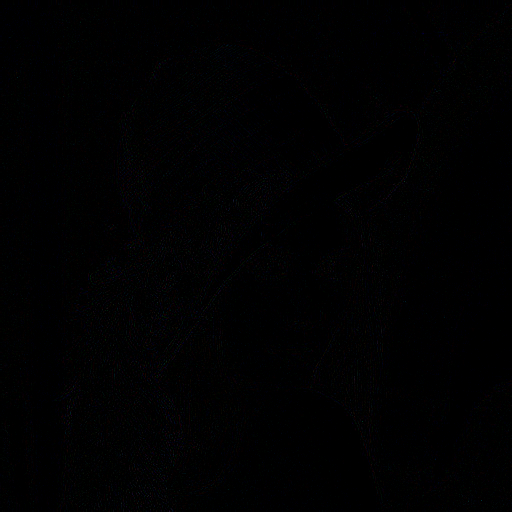
\includegraphics[scale=0.7]{./img/lenadif.png}
	\end{center}
\end{figure}
\begin{center}
\par Figura 7: Diferencia entre las figuras 5 y 6, imperceptible.
\end{center}

\begin{figure}[H]
	\begin{center}
	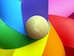
\includegraphics[scale=3]{./img/sample_1_in.jpg}
	\end{center}
\end{figure}
\begin{center}
\par Figura 8: \textit{Sample 1}, ampliada factor 3.
\end{center}

\begin{figure}[H]
	\begin{center}
	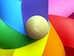
\includegraphics[scale=3]{./img/sample_1_alpha_1_out.jpg}
	\end{center}
\end{figure}
\begin{center}
\par Figura 9: \textit{Sample 1} tras la codificación, ampliada factor 3.
\end{center}

\begin{figure}[H]
	\begin{center}
	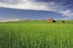
\includegraphics[scale=3]{./img/sample_3_in.jpg}
	\end{center}
\end{figure}
\begin{center}
\par Figura 10: \textit{Sample 2}, ampliada factor 3.
\end{center}

\begin{figure}[H]
	\begin{center}
	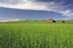
\includegraphics[scale=3]{./img/sample_3_alpha_1_out.jpg}
	\end{center}
\end{figure}
\begin{center}
\par Figura 11: \textit{Sample 2} tras la codificación, ampliada factor 3. Se pueden observar los bloques.
\end{center}

\section*{Anexo B: Variación del factor $alpha$.}

\begin{figure}[H]
	\begin{center}
	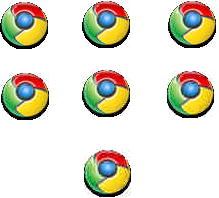
\includegraphics[scale=2.3]{./img/chromes.png}
	\end{center}
\end{figure}
\begin{center}
\par Figura 3: Codificación de varias imágenes del logo de \textit{Chrome} utilizando distintos 
valores de \textit{alpha}, variando ascendentemente de izquierda a derecha, arriba a abajo.
\end{center}




%----------------------------------------------------------------------

\section*{Anexo C: Tablas de resultados}

\begin{center}
	\begin{tabular}{|l || c | c | c | c|}
		\hline
		\textbf{Imagen} & \textbf{Tamaño en pixeles} & \textbf{Densidad de 0} & \textbf{Bits por pixel estimados} & \textbf{Error cuadrático medio}\\
		\hline
		\hline
		Lenna & 512x512 & 0.943 & 4.37 & 8\\
		Sample1 & 74x56 & 0.91 & 5.4 & 11\\
		Sample2 & 73x48 & 0.924 & 4.824 & 10\\
		chrome & 48x48 & 0.95 & 0.81 & 86\\
		facebook & 42x43 & 0.91 & 5.16 & 30\\
		\hline
	\end{tabular}
\end{center}
\begin{center}
Tabla 1: Compresión y errores de imágenes tras aplicar la codificación, usando $\alpha=1$.
\end{center}

\begin{center}
	\begin{tabular}{|l || c | c | c | c|}
		\hline
		\textbf{$\alpha$} & \textbf{Densidad de 0} & \textbf{Bits por pixel estimados} & \textbf{Error cuadrático medio}\\
		\hline
		\hline
		0.5 & 0.74 & 9.24 & 35\\
		0.75 & 0.78 & 8.28 & 64\\
		1 & 0.81 & 7.56 & 86\\
		1.3 & 0.835 & 6.96 & 133\\
		1.5 & 0.845 & 6.72 & 139\\
		2 & 0.87 & 6.12 & 181\\
		3 & 0.894 & 5.27 & 241\\
		\hline
	\end{tabular}
\end{center}
\begin{center}
Tabla 2: Compresión y errores de imágenes tras aplicar la codificación, usando $\alpha=1$.
\end{center}

\begin{center}
	\begin{tabular}{|l || c | c | c | c|}
		\hline
		\textbf{Nombre} & \textbf{Rellenado} & \textbf{Error cuadrático medio}\\
		\hline
		\hline
		dog & Bordes &  23\\
		dog & Ceros & 26\\
		facebook & Bordes & 17\\
		facebook & Ceros & 30\\
		\hline
	\end{tabular}
\end{center}
\begin{center}
Tabla 3: Comparación para distintos rellenados de imágenes, $\alpha=1$.
\end{center}

\section*{Anexo D: Matrices de ejemplo}

\begin{center}
\( G = 
\begin{pmatrix}

54.245 & -117 & -7.7 & -12.81 & -0.28 & 0.06 & 0.128 & 0.91 \\
26.113 & 6.13 & 0.73 & -0.1 & -5.13 & -0.9 & 0.1954 & 0.177 \\
-0.48 & 1.95 & -1.55 & -2.7 & -0.38 & -0.02 & 0.97 & 0.233 \\ 
3.969 & 2.86 & 0.37 & -0.47 & 0.385 & 0.01 & 0.027 & 0.377 \\ 
0.19 & 0.09 & 0.40 & 0.165 & -0.36 & 0.47 & 0.3 & -0.10 \\
-0.005 & -0.535 & -0.3 & -0.28 & 0.426 & -0.7 & 0.045 & -0.3 \\
0.41 & 0.59 & 0.125 & -0.38 & -0.16 & -0.157 & 0.33 & 0.086 \\
0.03 & -0.41 & -0.2 & 0.22 & 0.34 & 0.41 & 0.19 & 0.36 \\
\end{pmatrix}\)
\end{center}
\begin{center}
\par Ejemplo de una matriz salida, correspondiente a la luma del primer bloque de la imagen \textit{Sample 1}. Nótese 
que los números de mayor magnitud se encuentran en la zona superior izquierda.
\end{center}

\begin{center}
\( By = 
\begin{pmatrix}
3 & -11 & -1 & -1 & 0 & 0 & 0 & 0 \\
2 & 1 & 0 & 0 & 0 & 0 & 0 & 0 \\
0 & 0 & 0 & 0 & 0 & 0 & 0 & 0 \\ 
0 & 0 & 0 & 0 & 0 & 0 & 0 & 0 \\ 
0 & 0 & 0 & 0 & 0 & 0 & 0 & 0 \\
0 & 0 & 0 & 0 & 0 & 0 & 0 & 0  \\ 
0 & 0 & 0 & 0 & 0 & 0 & 0 & 0 \\
0 & 0 & 0 & 0 & 0 & 0 & 0 & 0 \\ 
\end{pmatrix}\)
\end{center}
\begin{center} Ejemplo de una matriz tras ser cuantificada, correspondiente al primer bloque de la luma de \textit{Sample 1}.
\end{center}

\section*{Anexo E: Código Octave}

\subsection{Pasaje de espacio de color de una imagen de RGB a $Y'C_bC_r$}

\VerbatimInput{../src/rgb_to_ybr.m}

\subsection{Pasaje de espacio $Y'C_bC_r$ a RGB. }

\VerbatimInput{../src/ybr_to_rgb.m}

\subsection{Pasaje de imagen a bloques $8x8$. }

\VerbatimInput{../src/img_to_blocks.m}

\subsection{Pasaje bloques a imagen. }

\VerbatimInput{../src/blocks_to_img.m}

\subsection{Transformada coseno discreta de bloque. }

\VerbatimInput{../src/disc_cos_transf.m}

\subsection{Antitransformada coseno discreta de bloque. }

\VerbatimInput{../src/disc_cos_antitransf.m}

\subsection{Cálculo del error cuadrático medio de una diferencia de imágenes. }

\VerbatimInput{../src/calc_error.m}

\subsection{Cálculo de la densidad de ceros. }

\VerbatimInput{../src/calc_zeros.m}

\subsection{Codificación y decodificación de una imagen.}

\VerbatimInput{../src/encode_and_decode.m}

\end{document}
